\documentclass[12pt,]{article}
\usepackage[utf8]{inputenc}
\usepackage[T1]{fontenc}
\usepackage{mathptmx}
\usepackage{geometry}
\usepackage{mathtools}
\usepackage[english]{babel}
\usepackage{graphicx}
\usepackage{stackengine}
\usepackage[os=win]{menukeys}
\usepackage{hyperref}
\usepackage{minted}
\usepackage{xcolor}
\usepackage{tikz}
\usepackage[yyyymmdd,hhmmss]{datetime}
\usepackage{etoolbox}

\patchcmd{\thebibliography}{\section*{\refname}}{}{}{}

\newcommand{\ShowOsVersion}{
	\immediate\write18{\unexpanded{foo=`uname -sro` && echo "${foo}" > tmp.tex}}
			\input{tmp}\immediate\write18{rm tmp.tex}
			}
			
\newcommand{\ShowTexVersion}{
			\immediate\write18{\unexpanded{foo=`pdflatex -version | head -n1 | cut -d' ' -f1,2` && echo "${foo}" > tmp.tex}}
	\input{tmp}\immediate\write18{rm tmp.tex}
}

\addto\captionsenglish{\renewcommand{\contentsname}{Daftar Isi}}

\hypersetup{
	colorlinks=true, %set true if you want colored links
	linktoc=all,     %set to all if you want both sections and subsections linked
	linkcolor=blue,  %choose some color if you want links to stand out
}

\geometry{
	legalpaper,
	left=15mm,
	right=10mm,
	top=10mm,
	bottom=15mm,
}

\title{\Large \bf
	Testing and Calibration Report\\
	\small{(Evaluation Purpose)}
}

\author{Achmadi ST MT}

\date{}

\definecolor{LightGray}{gray}{0.9}

\begin{document}
	\maketitle
	\thispagestyle{empty}
	
	\vspace*{600pt}
	\noindent This report written using: \\
	OS : \ShowOsVersion \\
	TeX : \ShowTexVersion \\
	Update: {\today} at \currenttime \\
	
	%%%%%%%%%%%%%%%%%%%%%%%%%%%%%%%%%%%%%%%%%%%%%%%%%%%%%%%%%%%%%%%%%
	
	\newpage
	\tableofcontents
	
	%%%%%%%%%%%%%%%%%%%%%%%%%%%%%%%%%%%%%%%%%%%%%%%%%%%%%%%%%%%%%%%%%
	
	\newpage
	\section{Proses Pengujian}
	
	\subsection{Persamaan}
	
	Persamaan yang digunakan untuk \textit{tone generation}:
	
	\[ Y = a.A.d.sin(2.\pi.f) \] dengan:
	\begin{itemize}
		\item \textbf{Y} adalah output sinus
		\item \textbf{a} adalah nilai atenuasi sebesar \textit{0.001}
		\item \textbf{A} adalah scaling amplitudo dari 1 hingga terkecil yang dapat didengar
		\item \textbf{d} adalah maksimum \textit{signed-32bit} positif sebesar \textit{32767}
		\item \textbf{$\pi$} adalah konstanta pi senilai \textit{3.141592653589793}
		\item \textbf(f) adalah rasio nilai antar index \textit{looping} dan panjang array.
		Panjang array berubah sesuai frekuensi yang akan dihasilkan
	\end{itemize}
	
	atau dalam format bahasa C:
	\begin{minted}[frame=lines,framesep=2mm,fontsize=\small,bgcolor=LightGray]{c}
#define DEFAULT_ATTEN 0.01
#define I2S_BUFF_SIZE 512

uint16_t sine_gen(double freq,double ampl){
  uint16_t buffsize = (uint16_t) I2S_BUFF_SIZE/freq;	

  for(i=0;i<buffsize;i++){
    ysin = DEFAULT_ATTEN*ampl*32767*sin(2*3.141592653589793*((double)i/(double)buffsize));
  }
}
	\end{minted}
	
	Implementasinya dapat dicek ulang di URL berikut:\\
	\url{https://github.com/VibrasticLab/pikoakustik/blob/stm32f401re_3pin/firmware/ht_audio.c}
	
	\subsection{Total Audio Output}
	
	Audio DAC (Digital Analog Converter) melalui jalur I2S pada \textit{Left-Channel}.
	Sinyal Output ditentukan dalam persamaan berikut\cite{Maxim}:
	
	\[Out = In + C + G\] dengan:
	
	\begin{itemize}
		\item \textbf{Out} adalah sinyal elektrik output (dBV)
		\item \textbf{In} adalah nilai array data I2S (dBFS)
		\item \textbf{C} adalah output minimum tanpa \textit{additional gain} (dB)
		\item \textbf{G} adalah additional amplifier gain (dB) 
	\end{itemize}

	dimana nilai \textbf{In} pada 0dBFS mengacu kepada 0dBV\cite{Maxim} dan nilai G dipilih yang terkecil yaitu 3dB mengacu kepada tabel berikut\cite{Maxim}:
	
	\begin{center}
		\begin{tabular}{ |c|c|c| } 
			\hline
			Pin-GAIN & Resistor & I2S GAIN \\ 
			\hline
			GND & 100K$\Omega$ & 15 dB \\ 
			GND & 0K$\Omega$ & 12 dB \\ 
			NC & NC & 9 dB \\ 
			VDD & 0K$\Omega$ & 6 dB \\ 
			VDD & 100K$\Omega$ & 3 dB \\ 
			\hline
		\end{tabular}\\
		\hfill \break
		Tabel 1: Pengaturan pin GAIN terhadap additional gain.
	\end{center}

	\newpage
	\subsection{Output Device}
	
	Dalam pengujian ini digunakan 4 (empat) merek headphone dengan spesifikasi resistansi (bukan impedansi) sebagaimana tabel berikut:
	
	\begin{center}
		\begin{tabular}{ |c|c|c| } 
			\hline
			Merek & Resistansi & Keterangan \\ 
			\hline
			Earphone & 20 $\Omega$ & \\ 
			\hline
			Kennion & 520 $\Omega$ & Volume Max \\ 
			\hline
			Miniso & 34 $\Omega$ & \\ 
			\hline
			Sanheiser & 320 $\Omega$ & Tercantum 300 $\Omega$ \\ 
			\hline
		\end{tabular}\\
		\hfill \break
	Tabel 2: Hasil ukur resistansi headphone yang akan diuji.
	\end{center}
	
	Metode pengukurannya adalah mengukur hambatan Jack TRS headphone pada pin Left-Ground (Tip-Sleeve) atau Right-Ground (Ring-Sleeve).
	Pengukuran menggunakan multimeter merek VIPER DT830B.
	
	\begin{figure}[!ht]
		\centering
		\includegraphics[width=150pt]{images/ohmcheck}
		\caption{Ilustrasi pengukuran resistansi headphone}
	\end{figure}

	\subsection{Setup Pengujian}
	
	Setup pengujian secara ringkas adalah:
	\begin{enumerate}
		\item Microphone merek \textbf{dbx} dipasang di sisi kiri dan kanan headphone yang diuji.
		Digunakan karpet sebagai penghalang kanan-kiri.
		
		\item Jack Audio 3.5m dari headphone disambungkan ke unit Audiometri.
		Sambungkan pula kabel USB dari unit Audiometri.
		
		\item Output microphone disambungkan ke audio interface \textbf{Focusrite Scarlett 18i8}.
		Digunakan Input Gain pada nilai maximum.
		
		\item Data USB dari audio interface dihubungkan ke laptop.
		Sambungkan pula USB dari unit Audiometri ke laptop.
		
		\item Software audio interface di laptop adalah \textbf{Realtime Analyzer} versi 5.2.0.26 yang
		merupakan paket dari software \textbf{DSSF3} buatan Yoshimasha Electronic Inc.
		Pembobotan yang digunakan adalah \textbf{A-Weighting}.
		
		\item Unit Audiometri kemudian dinyalakan dengan tegangan 5v dari USB laptop.
		
		\begin{figure}[!ht]
			\centering
			\includegraphics[width=150pt]{images/setup0}
			\includegraphics[width=150pt]{images/setup1}
			\includegraphics[width=150pt]{images/setup2}
			\caption{Setup pengujian pada langkah 1, 2, dan 3}
		\end{figure}
		
		\newpage
		\item Jalankan serial terminal untuk berkomunikasi antara laptop dan unit Audiometri.
		Software serial terminal yang digunakan adalah \textbf{minicom} pada port \textit{/dev/ttyACM0} atau \textit{/dev/ttyACM1}.
		
		\item Perintah yang dikirim ke unit Audiometri untuk menjalankan fungsi \textit{tone generator}.
\begin{minted}[frame=lines,framesep=2mm,fontsize=\small,bgcolor=LightGray]{bash}
tone <0/1> <frequency> <amplitude>
\end{minted}
		dengan:
		\begin{itemize}
			\item \textbf{0/1} adalah pilihan channel Left (\textbf{0}) atau Right (\textbf{1}).
			
			\item \textbf{frequency} adalah skala ukuran array untuk menentukan frekuensi.
			Frekuensi yang tersedia (dalam Hz) adalah \textbf{250, 500, 1000, 2000, 4000} dan \textbf{8000}.
			Skala frekuensi yang bersesuaian adalah \textbf{0.625, 1.25, 2.5, 5, 10} dan \textbf{20}.
			
			\item \textbf{amplitude} adalah skala amplitudo yang akan dikirim.
			Skala yang digunakan adalah \textbf{1, 0.5, 0.25, 0.125, 0.0625, 0.0312, 0.0156, 0.0078} dan \textbf{0.0039}.
			Nilai skala \textbf{0.0031} adalah batas minimum dimana dibawah skala itu hanya akan terdengar noise tanpa tone.
		\end{itemize}
		
		sehingga contoh perintahnya untuk tone frekuensi 500Hz dan skala amplitudo 1 di \textit{Left channel}.
\begin{minted}[frame=lines,framesep=2mm,fontsize=\small,bgcolor=LightGray]{bash}
tone 0 1.25 1
\end{minted}

		\begin{figure}[!ht]
			\centering
			\includegraphics[width=200pt]{hasil/test/cmdtest}
			\includegraphics[width=200pt]{hasil/test/test}
			\caption{Contoh perintah dan hasil pada analyzer}
		\end{figure}
	\end{enumerate}

	\subsection{Hasil Tes}
	
	Dengan asumsi bahwa chip Audio DAC pada Left dan Right channel adalah chip yang sama,
	kemudian mendapat sinyal array I2S yang sama pula,
	maka pengujian ini dilakukan hanya pada Left Channel saja.
	
	Berikutnya akan dijabarkan hasil uji setiap headphone.
	
  	\subsubsection{Miniso}
	
	Hasil pengujian amplitudo
	
	\begin{figure}[!ht]
		\centering
		\includegraphics[width=250pt]{hasil/miniso/max_freq}
		\includegraphics[width=250pt]{hasil/miniso/each_freq}
		\caption{amplitudo maksimal setiap frekuensi (kiri) dan di setiap skala frekuensi (kanan)}
	\end{figure}
	
	\newpage
	\section{Referensi}
	\label{}
	
	\bibliographystyle{IEEEtran}
	\bibliography{/home/achmaday/Documents/BibTex/library.bib}
		
\end{document}